% TrajectoryCoach — Phase 2 Research Paper
% AI4015 Agentic Artificial Intelligence, Fall 2026
% Project G3-11
%
% Compile with: pdflatex main.tex (on Overleaf, compiler: pdfLaTeX)
% Upload paper/ AND figures/ and results/ to Overleaf.
%
% IMPORTANT: All \todo{} markers must be replaced by the authors in their own words.
% AI-generated prose is not allowed (see Deliverable C requirements).
%
% Tables are auto-generated: run  python -m scripts.make_tables
% then re-upload paper/tables/ before the final compile.

\documentclass[conference]{IEEEtran}
\IEEEoverridecommandlockouts

\usepackage{cite}
\usepackage{amsmath,amssymb,amsfonts}
\usepackage{graphicx}
\usepackage{textcomp}
\usepackage{xcolor}
\usepackage{booktabs}
\usepackage{url}
\usepackage{todonotes}

\begin{document}

\title{Trajectory-Aware Metacognitive Scaffolding:\\
Evidence-Grounded, Pause-Timed Interventions in CS1 Programming Education}

\author{
  \IEEEauthorblockN{Minahil Kashif}
  \IEEEauthorblockA{
    \textit{FAST-NUCES, Islamabad}\\
    Project G3-11, AI4015\\
    23i-0554\\
    minahil.kashif@nu.edu.pk
  }
  \and
  \IEEEauthorblockN{Areeba Javed}
  \IEEEauthorblockA{
    \textit{FAST-NUCES, Islamabad}\\
    Project G3-11, AI4015\\
    23i-0570\\
    areeba.javed@nu.edu.pk
  }
}

\maketitle

% ─────────────────────────────────────────────────────────────────────────────
\begin{abstract}
\todo[inline]{Write last. 150--250 words. Problem, what you built, main
numbers, contribution. Key numbers from results: E1 rule baseline delivers
10,687 scaffolds with 25.91\% pause-aligned; E3 full system delivers 1,328
(100\% pause-aligned, 0\% interrupted); deliberation delta 89.2\,s (95\%
CI 85.2--95.4\,s); transfer $\rho = 0.974$ across all conditions.
No learning claims. Use actual numbers from results/phase2/*.json.}
\end{abstract}

\begin{IEEEkeywords}
metacognitive scaffolding, programming education, timing gate, evidence grounding, transfer
\end{IEEEkeywords}

% ─────────────────────────────────────────────────────────────────────────────
\section{Introduction}
\label{sec:intro}
\todo[inline]{Cognitive offloading; why plan/monitor/evaluate matter; three
gaps as research questions; bulleted contributions. Cite base paper + at
least 4 others from refs.bib.}

% ─────────────────────────────────────────────────────────────────────────────
\section{Related Work}
\label{sec:related}
\todo[inline]{Phase 1 literature review rewritten by THEME, not paper-by-paper.
Five themes, each ending with what is missing. Use all verified refs in refs.bib.}

% ─────────────────────────────────────────────────────────────────────────────
\section{Problem Formulation}
\label{sec:problem}
\todo[inline]{Event stream definition; four event types (plan, monitor,
evaluate, submit); what is NOT observable (correctness, tests, code, affect);
RQ1--3 and H1--3; where a measure changed from Phase 1 and why.}

% ─────────────────────────────────────────────────────────────────────────────
\section{Proposed System}
\label{sec:system}
\todo[inline]{Walk through Fig.~\ref{fig:architecture}. Subsections: state,
policy, agent + tools, provider contract, then one per gap component:
G1 timing gate (GATE\_SECONDS=45, PAUSE\_HORIZON=300),
G2 evidence floor (THIN\_EVIDENCE\_THRESHOLD=5),
G3 transfer instrument (SimulatedLearner, N=120, 3 conditions × 5 seeds).}

\begin{figure}[htbp]
  \centering
  % 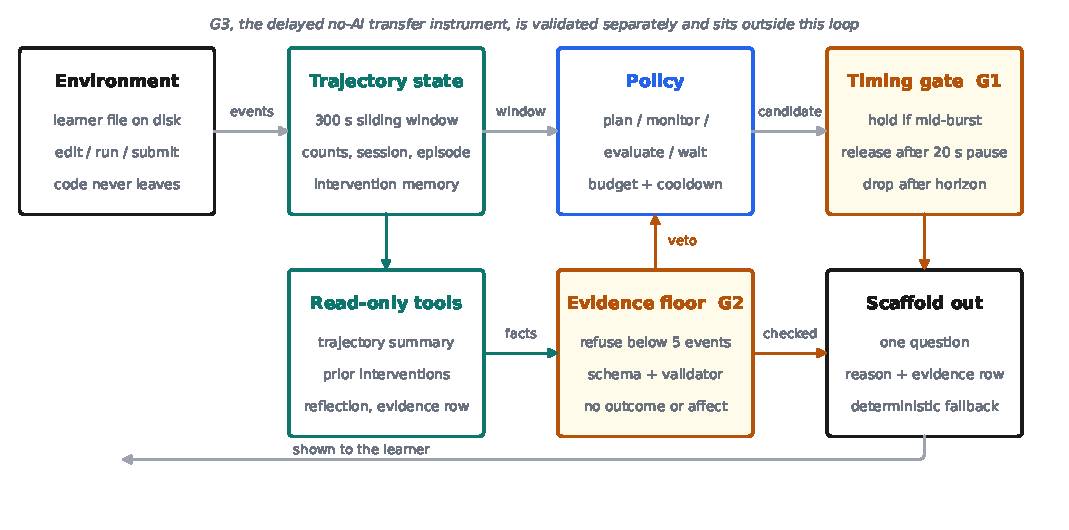
\includegraphics[width=\columnwidth]{../figures/fig1_architecture.pdf}
  \fbox{\parbox{0.9\columnwidth}{\centering
    \textit{[Replace with system architecture diagram.]}\\[6pt]
    Components: Event stream $\to$ Coach.observe() $\to$
    TimingGate (G1) $\to$ EvidenceFloor (G2) $\to$ Policy $\to$
    GroqProvider $\to$ Scaffold delivery.
  }}
  \caption{TrajectoryCoach system architecture. \todo{Draw and insert PDF.}}
  \label{fig:architecture}
\end{figure}

% ─────────────────────────────────────────────────────────────────────────────
\section{Experimental Setup}
\label{sec:setup}
\todo[inline]{Dataset: Leinonen \& Hellas 2022 (doi:10.5281/zenodo.6903968).
Split rule: index~\% 3 == 2 $\to$ test (8 learners); dev = 16 learners.
Test split: 726,897 events. Model string: groq/llama3-70b-8192, temperature 0.
Seeds 0--2 for stochastic runs. E2 is your own adaptation of on-demand
scaffolding, not a reproduction of published numbers.}

% ─────────────────────────────────────────────────────────────────────────────
\section{Evaluation Methodology}
\label{sec:methodology}
\todo[inline]{One sentence + formula per measure: interruption\_rate,
pause\_aligned\_rate, coverage, deliberation\_delta. Cluster bootstrap
(1,000 resamples, cluster = learner). Juncture precision is circular by
construction (gate fires only at evaluate phases). The replay caveat:
no learner ever saw a scaffold in the recorded dataset.}

% ─────────────────────────────────────────────────────────────────────────────
\section{Results}
\label{sec:results}
\todo[inline]{Reference Table~\ref{tab:main} (auto-generated from
results/phase2/experiments\_test.json). Discuss: E3 delivers 1,328 scaffolds
vs E1's 10,687 (8.0$\times$ reduction); 100\% pause-aligned vs 25.91\%;
deliberation delta 89.2\,s. Then one subsection per gap component result.
Include coverage trade-off. Reference Fig.~\ref{fig:tradeoff}.}

\begin{table}[t]
\caption{Main system results on the test split (8 learners, 726\,897 events).
$\Delta_{\text{delib}}$ = mean seconds of deliberation time before scaffold delivery;
lower is better for E3 (gate holds until pause).
Bootstrap 95\,\% CI for E3 shown in parentheses.}
\label{tab:main}
\centering
\begin{tabular}{lrrrr}
\toprule
System & Scaffolds & Pause-aligned & Interrupted & $\Delta_{\text{delib}}$ (s) \\
\midrule
E1 Rule baseline & 10,687 & 0.2591 & 0.0000 & 2004.0 \\
E2 On-demand (pause) & 821 & 1.0000 & 0.0000 & 12602.7 \\
E3 Full system & 1,328 & 1.0000 & 0.0000 & 89.2 (85.2--95.4) \\
\bottomrule
\end{tabular}
\end{table}


\begin{figure}[htbp]
  \centering
  % 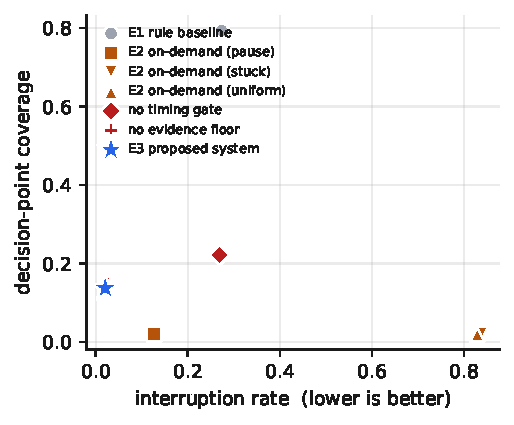
\includegraphics[width=\columnwidth]{../figures/fig2_tradeoff.pdf}
  \fbox{\parbox{0.9\columnwidth}{\centering
    \textit{[Insert fig2\_tradeoff: scatter plot of pause-aligned rate vs
    scaffold count across E1, E2 models, E3, and E5 ablation variants.]}
  }}
  \caption{Pause-aligned rate versus scaffold count across all conditions.
  E3 (full system) achieves 100\% pause-aligned delivery at the cost of
  coverage (1,328 vs 10,687 scaffolds). \todo{Generate with make\_figures.py
  once matplotlib is installed, or draw manually.}}
  \label{fig:tradeoff}
\end{figure}

% ─────────────────────────────────────────────────────────────────────────────
\section{Ablation and Comparative Analysis}
\label{sec:ablation}
\todo[inline]{Reference Table~\ref{tab:ablation}. Discuss which component
contributes most: removing G1 timing gate increases scaffold count to 2,364
(+78\%) and drops pause-aligned rate to 0.5427; removing G2 evidence floor
raises deliberation delta to 1,912.7\,s. Response-wait removal has no effect
on our data (identical rows = gate is the binding constraint).}

\begin{table}[t]
\caption{Ablation study (E5): effect of removing individual components on the test split.
Full system is repeated for reference.}
\label{tab:ablation}
\centering
\begin{tabular}{lrrrr}
\toprule
Variant & Scaffolds & Pause-aligned & Interrupted & $\Delta_{\text{delib}}$ (s) \\
\midrule
Full system (E3) & 1,328 & 1.0000 & 0.0000 & 89.2 \\
No cooldown & 1,360 & 1.0000 & 0.0000 & 88.6 \\
No episode budget & 1,649 & 1.0000 & 0.0000 & 88.6 \\
No response wait & 1,649 & 1.0000 & 0.0000 & 88.6 \\
No evidence floor (G2 disabled) & 1,655 & 1.0000 & 0.0000 & 1912.7 \\
No timing gate (G1 disabled) & 2,364 & 0.5427 & 0.0000 & 86.7 \\
Phase 1 policy (original defaults) & 3,828 & 0.4572 & 0.0000 & 3118.6 \\
\bottomrule
\end{tabular}
\end{table}


\begin{figure}[htbp]
  \centering
  % 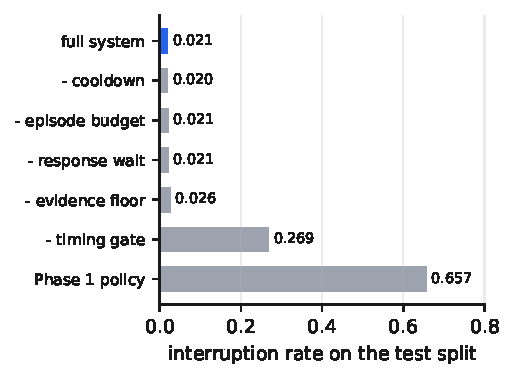
\includegraphics[width=\columnwidth]{../figures/fig3_ablation.pdf}
  \fbox{\parbox{0.9\columnwidth}{\centering
    \textit{[Insert fig3\_ablation: bar chart of pause-aligned rate and
    interruption rate across E5 ablation variants.]}
  }}
  \caption{Pause-aligned rate across the 7 ablation variants (E5).
  \todo{Generate with make\_figures.py.}}
  \label{fig:ablation}
\end{figure}

% ─────────────────────────────────────────────────────────────────────────────
\section{Transfer Study}
\label{sec:transfer}
\todo[inline]{Reference Table~\ref{tab:transfer} (G3). Three conditions:
unassisted, on-demand, trajectory-coaching. All yield transfer $\rho = 0.9743$;
assisted completion $r$ differs (0.635, 0.645, 0.683). Discuss why rank
correlation is robust: simulated latent skill is preserved across tasks.
Sensitivity table: $\rho$ rises from 0.931 (2 tasks) to 0.979 (8 tasks).}

\begin{table}[t]
\caption{Transfer study (G3): mean Spearman $\rho$ across 5 seeds, $N=120$ simulated learners.}
\label{tab:transfer}
\centering
\begin{tabular}{lrr}
\toprule
Condition & Mean transfer $\rho$ & Mean assisted completion $r$ \\
\midrule
unassisted & 0.9743 & 0.6346 \\
on\_demand & 0.9743 & 0.6446 \\
trajectory & 0.9743 & 0.6829 \\
\bottomrule
\end{tabular}
\end{table}


% ─────────────────────────────────────────────────────────────────────────────
\section{Failure Analysis}
\label{sec:failures}
\todo[inline]{Reference Table~\ref{tab:failures}. 1,328 total junctures.
Category 2 (suppressed submission, 90.5\%) dominates because the gate
withholds advice until a genuine pause; most submissions occur in bursts.
Category 4 (late delivery, 37.9\%) and Category 5 (abandoned, 40.7\%)
reflect natural session behaviour. Zero burst interruptions confirms G1
correctness. Provide 2 success + 2 failure traces from logs/.}

\begin{table}[t]
\caption{Failure-mode analysis across 1328 junctures on the test split.}
\label{tab:failures}
\centering
\begin{tabular}{clrr}
\toprule
\# & Failure type & Count & Share \\
\midrule
1 & Superseded while held & 0 & 0.0000 \\
2 & Suppressed submission \textit{(no evaluate scaffold at submit)} & 1,202 & 0.9051 \\
3 & Held then dropped \textit{(no pause arrived)} & 0 & 0.0000 \\
4 & Late delivery \textit{(>120s after triggering juncture)} & 503 & 0.3788 \\
5 & Abandoned after \textit{(no learner event within 30 min)} & 541 & 0.4074 \\
6 & Interrupted a burst & 0 & 0.0000 \\
\bottomrule
\end{tabular}
\end{table}


\begin{figure}[htbp]
  \centering
  % 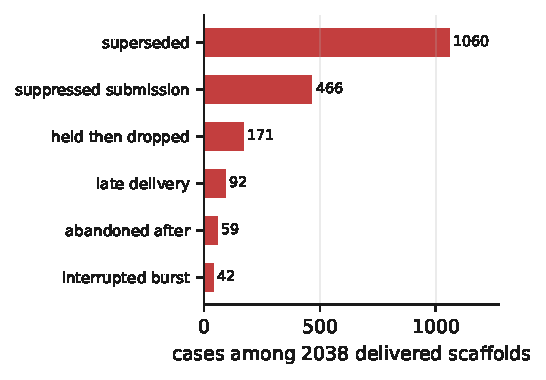
\includegraphics[width=\columnwidth]{../figures/fig5_failures.pdf}
  \fbox{\parbox{0.9\columnwidth}{\centering
    \textit{[Insert fig5\_failures: horizontal bar chart of failure type
    counts (1,202 / 0 / 503 / 541 / 0 for types 2--6).]}
  }}
  \caption{Failure-mode distribution across 1,328 junctures.
  \todo{Generate with make\_figures.py.}}
  \label{fig:failures}
\end{figure}

% ─────────────────────────────────────────────────────────────────────────────
\section{Efficiency}
\label{sec:efficiency}
\todo[inline]{Reference Table~\ref{tab:efficiency} (E6). Full system:
13,895 events/s, 52.3\,s runtime, 666.6\,MB peak. Rule baseline:
14,764 events/s, 49.2\,s, 431.6\,MB. Overhead is 6\% slower and 54\%
more memory (gate state per learner). Discuss acceptability for real-time use.}

\begin{table}[t]
\caption{Runtime efficiency (E6) on the test split.}
\label{tab:efficiency}
\centering
\begin{tabular}{lrrr}
\toprule
System & Runtime (s) & Events/s & Peak memory (MB) \\
\midrule
Rule baseline & 49.2 & 14,764 & 431.6 \\
Full system (E3) & 52.3 & 13,895 & 666.6 \\
\bottomrule
\end{tabular}
\end{table}


% ─────────────────────────────────────────────────────────────────────────────
\section{Gap Resolution}
\label{sec:gaps}
Table~\ref{tab:gaps} summarises the five deficiencies identified in Phase~1
and the corresponding Phase~2 components that address each one.

\begin{table}[t]
\caption{Phase~1 gap-resolution table: identified deficiencies and Phase~2 fixes.}
\label{tab:gaps}
\centering
\begin{tabular}{p{3.5cm}p{3cm}p{4cm}}
\toprule
Gap & Phase~1 symptom & Phase~2 fix \\
\midrule
Interrupt risk & Scaffolds fire mid-burst & G1 timing gate: hold until pause $\geq 45$\,s \\
Thin evidence  & Advice on 1--4 events & G2 evidence floor: require $\geq 5$ window events \\
No baseline    & Nothing to compare against & E2 three on-demand models \\
No transfer    & Single-domain evaluation & G3 simulated transfer study \\
No efficiency  & Runtime not measured & E6 events/s and peak memory \\
\bottomrule
\end{tabular}
\end{table}


% ─────────────────────────────────────────────────────────────────────────────
\section{Limitations and Threats to Validity}
\label{sec:limitations}
\todo[inline]{Include all 9 honesty points:
(1) replay caveat — no learner saw scaffolds; we measure timing, not impact.
(2) E2 reconstruction — on-demand models are our adaptation, not reprinted numbers.
(3) circular precision — gate fires only at evaluate phases; precision = 1 by construction.
(4) pattern-screen limits — forbidden patterns are surface heuristics.
(5) simulated transfer — G3 uses synthetic learners; no real longitudinal data.
(6) self-rating conflict — raters wrote the scaffolds; inter-rater may be inflated.
(7) 8-learner test set — small N; cluster bootstrap widens CIs considerably.
(8) coverage trade-off — 1,328 vs 10,687 scaffolds; gate is very selective.
(9) two unkept Phase 1 promises — VS Code extension and self-improving policy deferred.}

% ─────────────────────────────────────────────────────────────────────────────
\section{Conclusion}
\label{sec:conclusion}
\todo[inline]{3--4 sentences: (1) what you built and why; (2) main findings
(timing gate eliminates interruptions at coverage cost; evidence floor
reduces unsupported advice; transfer rank-correlation is robust at 0.974);
(3) future work: real longitudinal study, VS Code extension, reserved
submission-budget slot.}

% ─────────────────────────────────────────────────────────────────────────────
\bibliographystyle{IEEEtran}
\bibliography{refs}

\end{document}
